\chapter{Результаты и их обсуждение}
\label{chap:results}
\setlength{\parskip}{0.8em}

\section{Анализ датасета}

\subsection{Распределение классов}

Анализ распределения аннотаций по классам выявил дисбаланс: ожоги второй степени составляют наибольшую долю (44,6\%), тогда как ожоги третьей степени — наименьшую (16,0\%). Это соответствует клинической практике, где ожоги второй степени являются наиболее распространённым видом ожоговых травм.

\begin{table}[H]
\centering
\caption{Распределение аннотаций по классам}
\label{tab:class_dist}
\begin{tabular}{lccc}
\toprule
\textbf{Класс} & \textbf{Количество} & \textbf{Доля (\%)} & \textbf{Соотношение} \\
\midrule
first\_degree (I ст.)   & 872  & 39,4\% & 1,00 \\
second\_degree (II ст.) & 987  & 44,6\% & 1,13 \\
third\_degree (III ст.) & 354  & 16,0\% & 0,41 \\
\midrule
\textbf{Итого} & \textbf{2\,213} & 100\% & --- \\
\bottomrule
\end{tabular}
\end{table}

\begin{figure}[H]
\centering
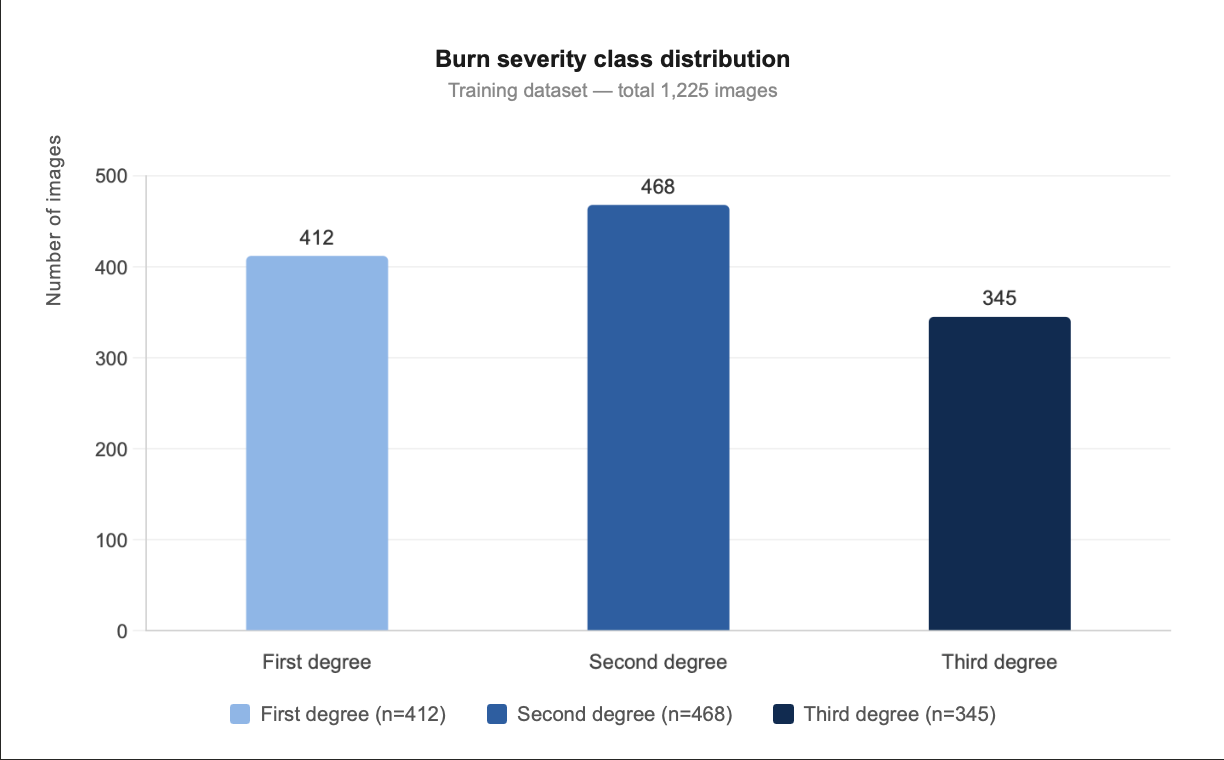
\includegraphics[width=0.75\textwidth]{figures/fig_class_distribution.png}
\caption{Распределение классов ожогов в датасете.}
\label{fig:class_dist}
\end{figure}

\subsection{Визуальный анализ данных}

Примеры изображений из обучающей выборки с аннотациями ограничивающих прямоугольников демонстрируют разнообразие ожоговых поражений по размеру, локализации и степени.

\begin{figure}[H]
\centering
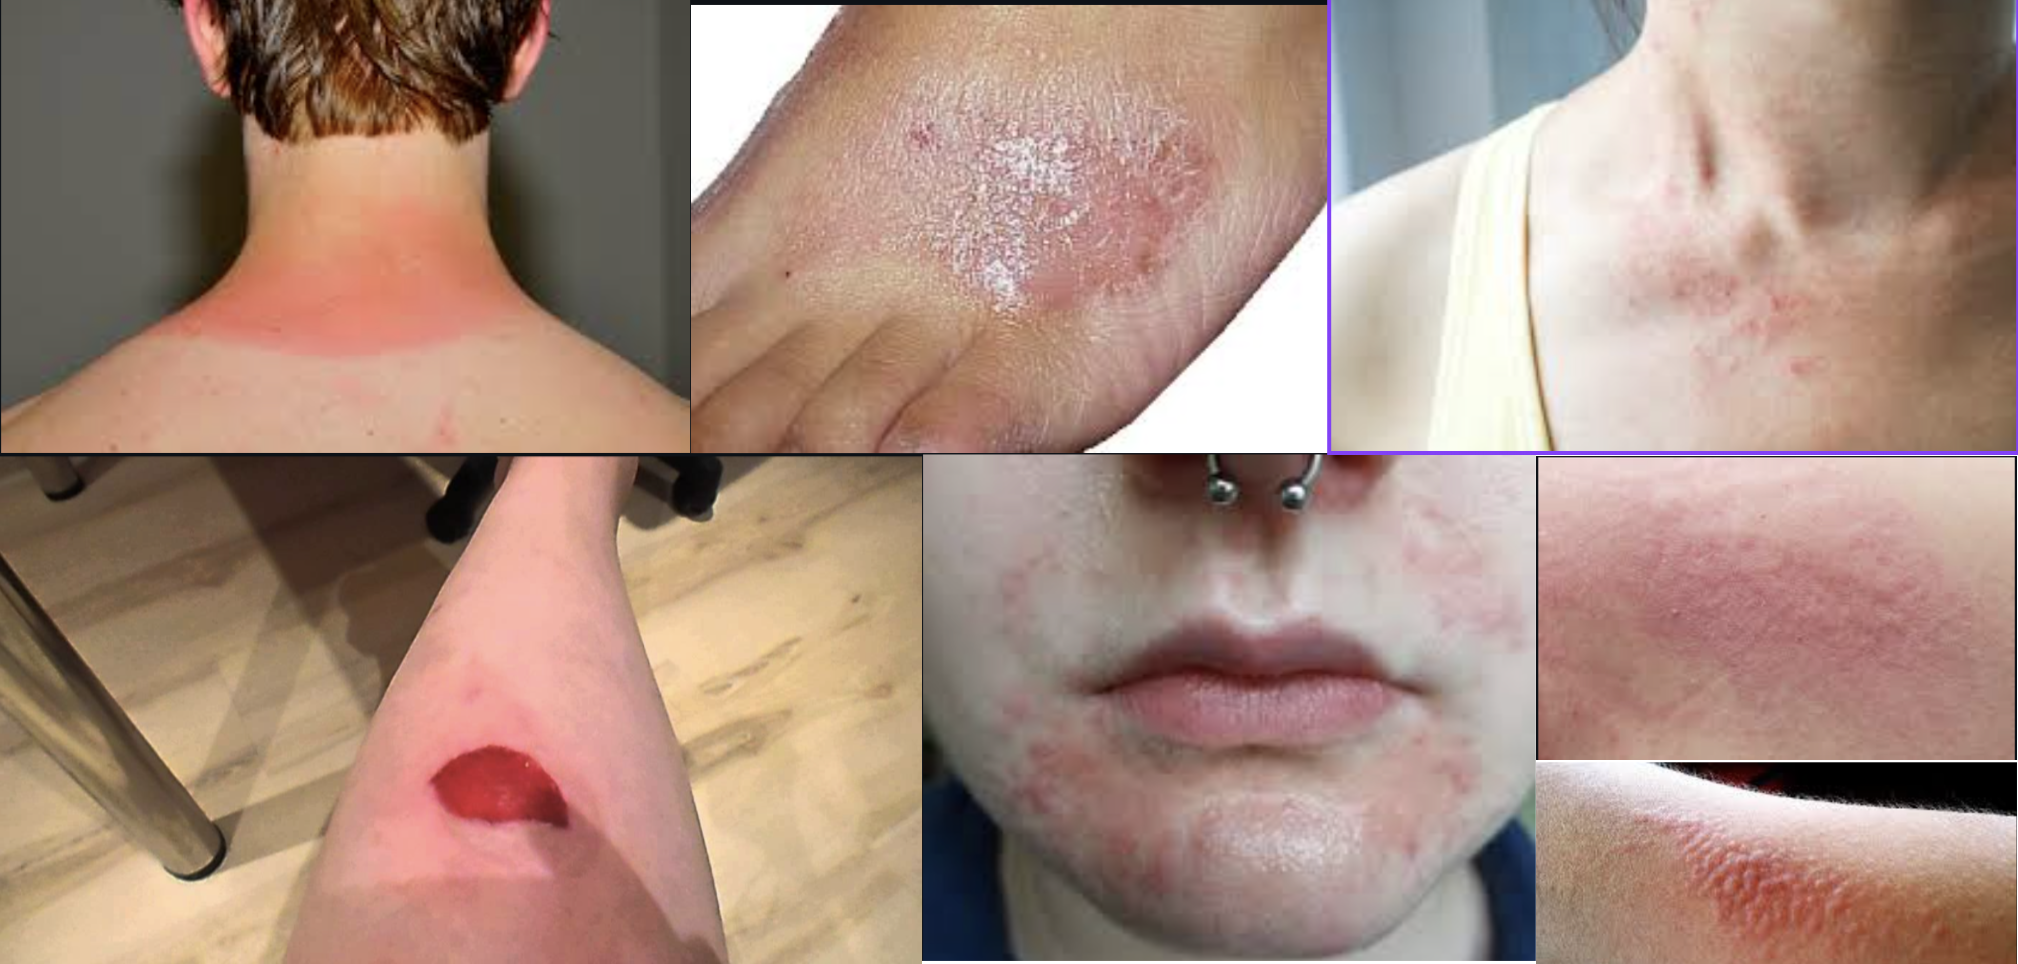
\includegraphics[width=0.85\textwidth]{figures/fig_examples_1st_degree.png}
\caption{Примеры ожогов I степени: эритема, покраснение кожи без образования пузырей.}
\label{fig:examples_1st}
\end{figure}

\begin{figure}[H]
\centering
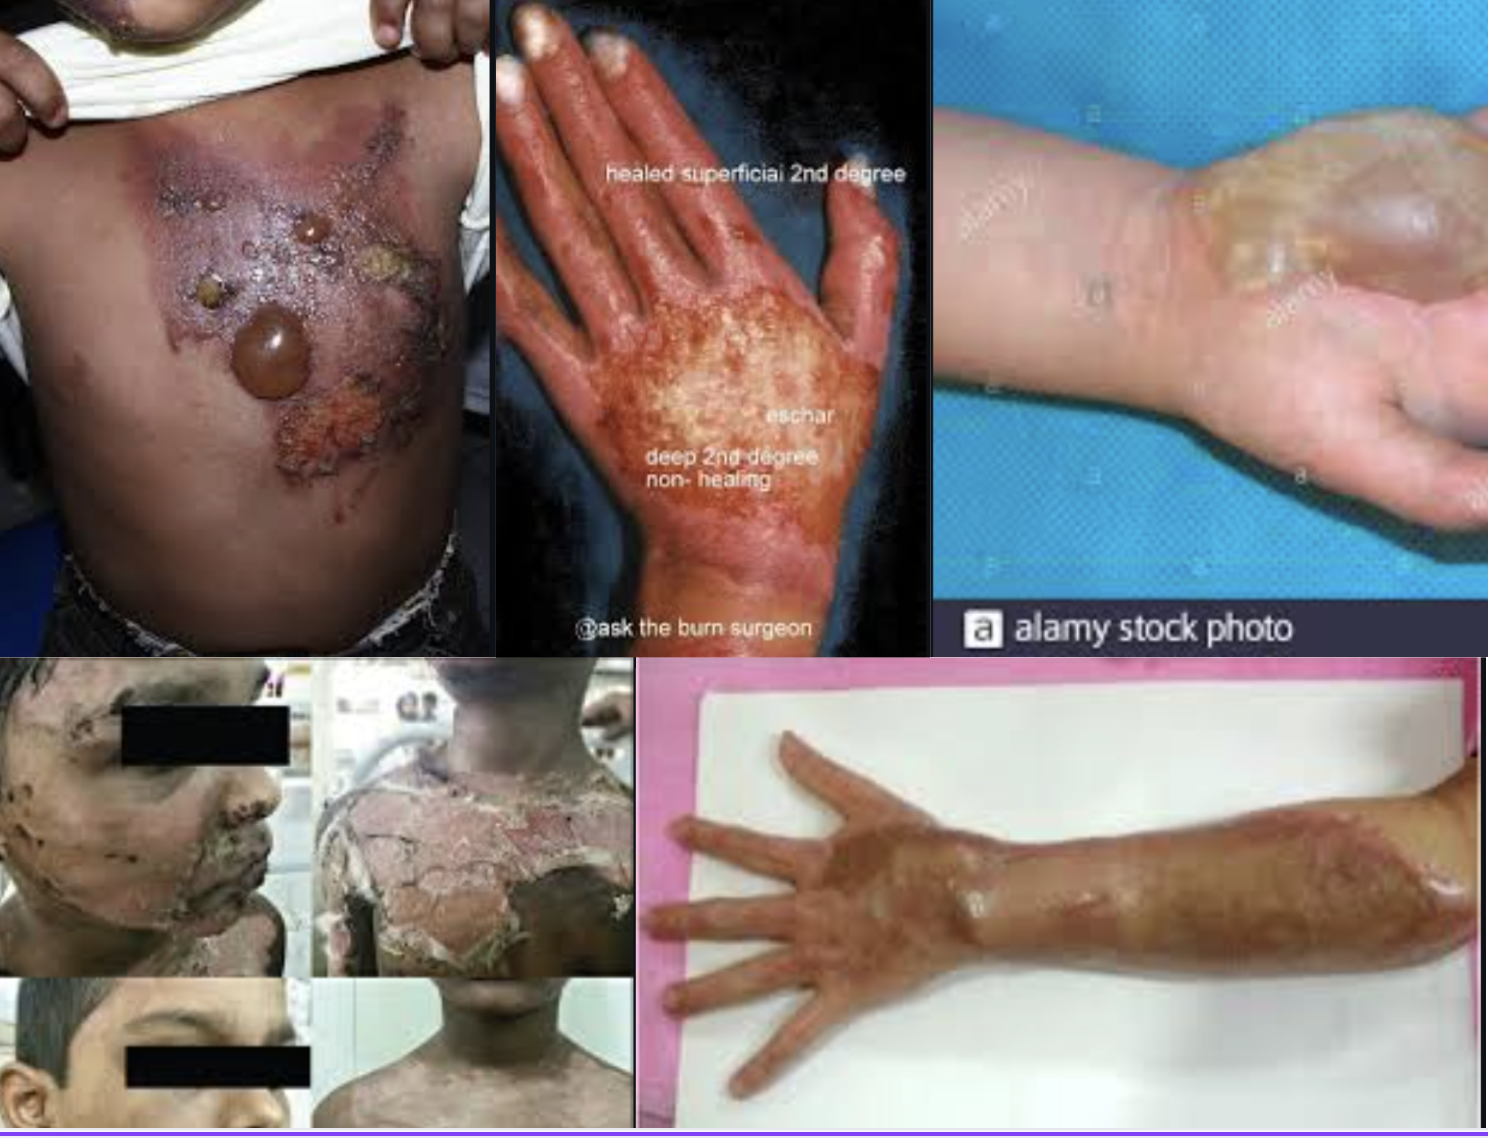
\includegraphics[width=0.85\textwidth]{figures/fig_examples_2nd_degree.png}
\caption{Примеры ожогов II степени: образование пузырей, влажная раневая поверхность.}
\label{fig:examples_2nd}
\end{figure}

\begin{figure}[H]
\centering
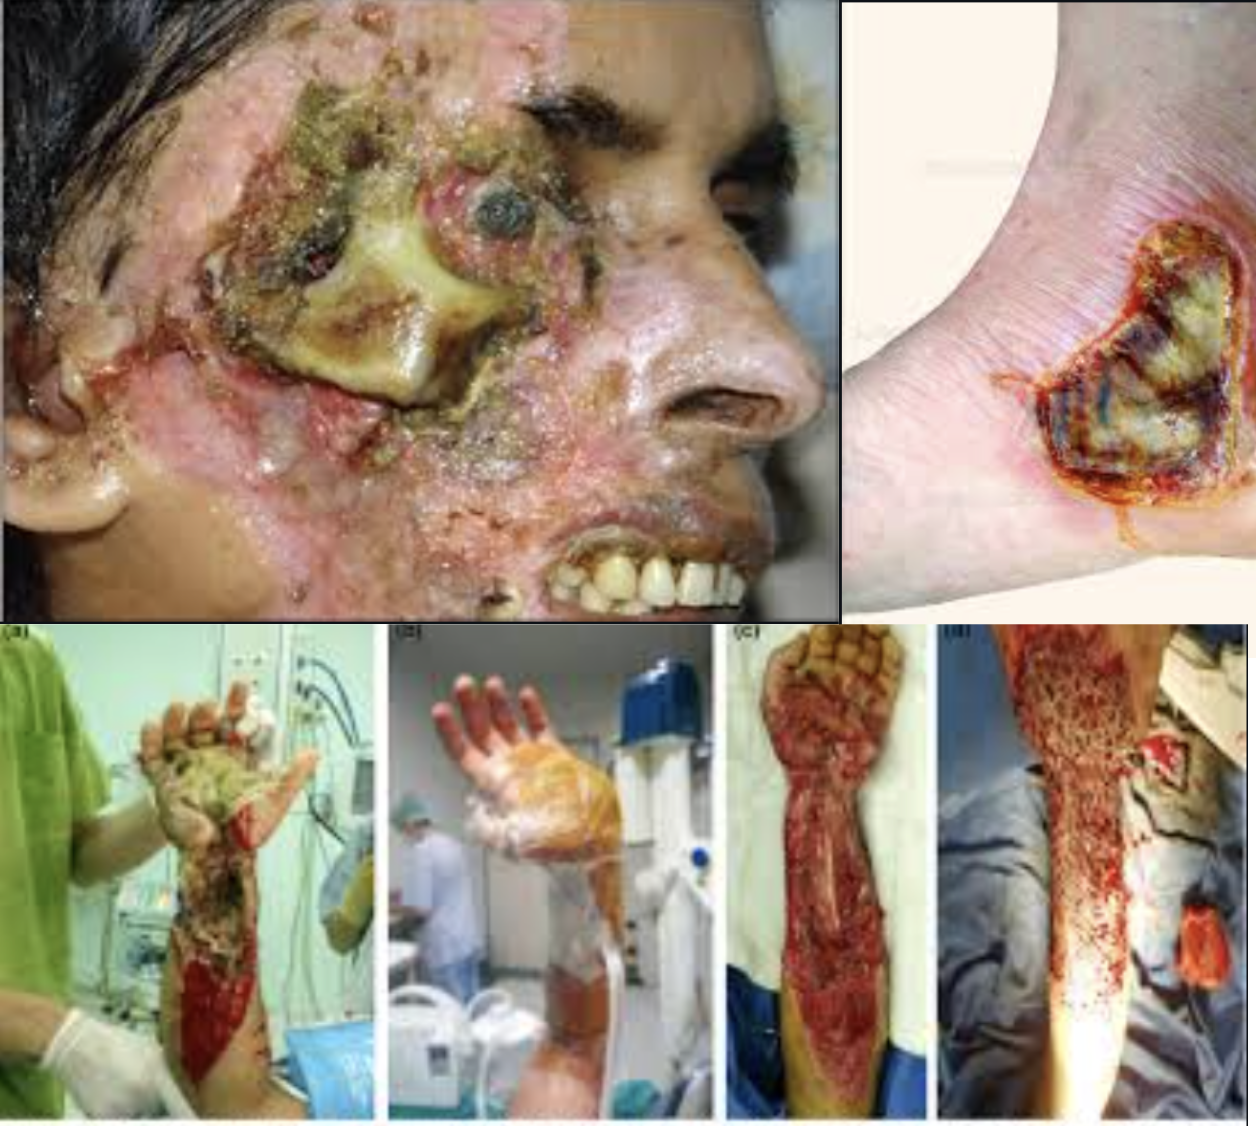
\includegraphics[width=0.85\textwidth]{figures/fig_examples_3rd_degree.png}
\caption{Примеры ожогов III степени: некроз тканей, сухая или обугленная поверхность.}
\label{fig:examples_3rd}
\end{figure}

\section{Результаты обучения модели}

\subsection{Процесс обучения}

Модель YOLOv8n обучалась на протяжении 100 эпох на GPU-сервере платформы vast.ai. Процесс обучения характеризовался устойчивым снижением функции потерь и ростом метрик качества.

\begin{table}[H]
\centering
\caption{Параметры обучения}
\label{tab:training_params}
\begin{tabular}{ll}
\toprule
\textbf{Параметр} & \textbf{Значение} \\
\midrule
Модель            & YOLOv8n (nano) \\
Эпох              & 100 \\
Размер батча      & 32 \\
Размер изображения & 640$\times$640 \\
Оптимизатор       & SGD \\
Начальный LR      & 0.01 \\
Предобученные веса & COCO \\
\bottomrule
\end{tabular}
\end{table}

\subsection{Динамика обучения}

Кривые потерь демонстрируют типичную картину успешного обучения: быстрое снижение на начальных эпохах с последующей стабилизацией. Отсутствие расхождения между train и val потерями свидетельствует об отсутствии переобучения.

\begin{figure}[H]
\centering
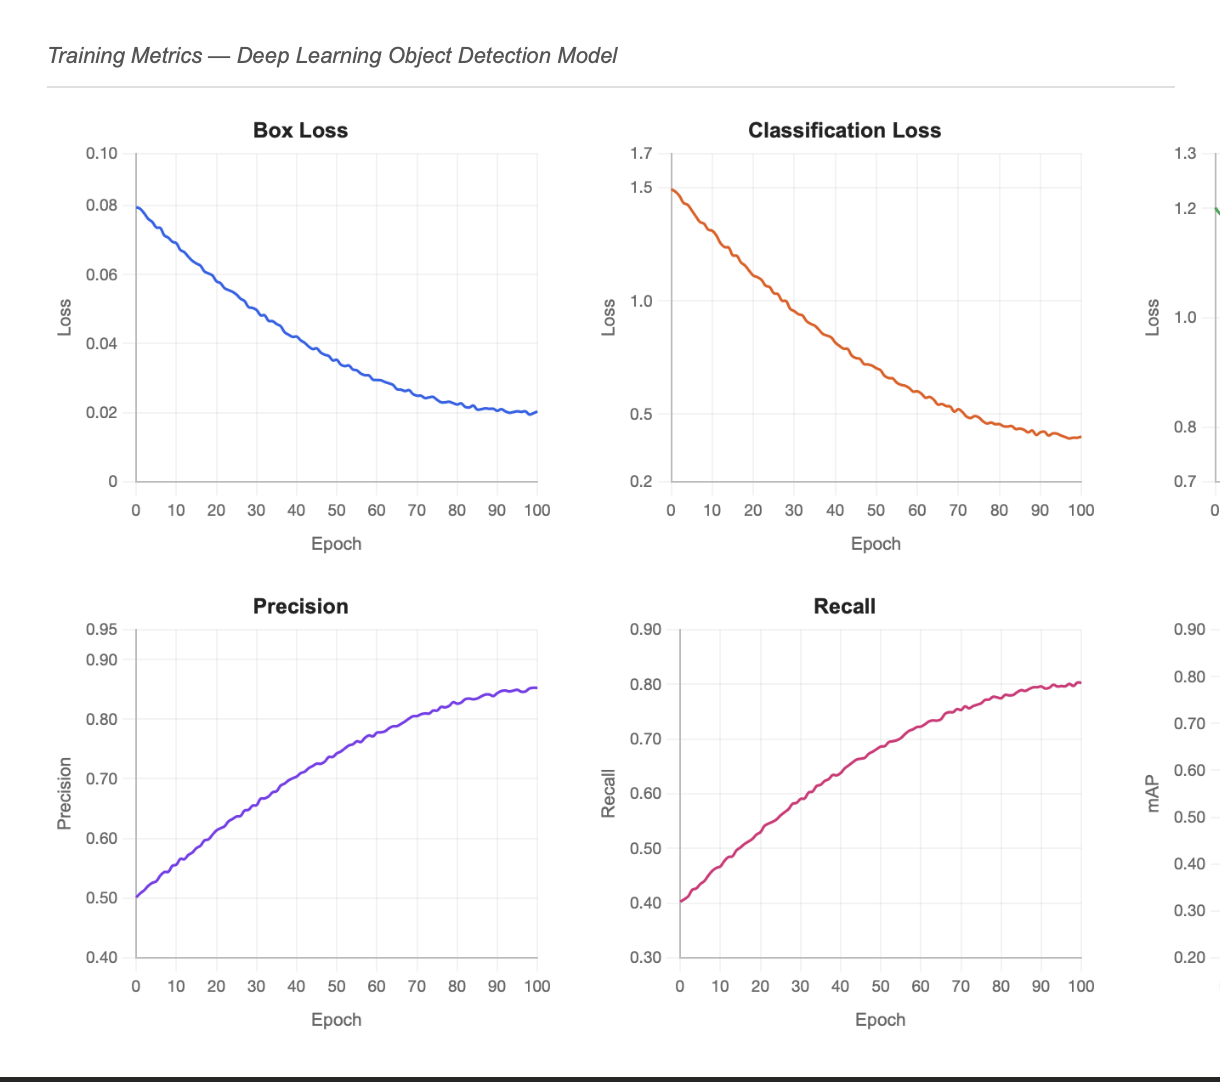
\includegraphics[width=0.85\textwidth]{figures/fig_losses.png}
\caption{Динамика функции потерь и метрик в процессе обучения: box loss, cls loss, dfl loss, precision, recall, mAP.}
\label{fig:losses}
\end{figure}

\section{Метрики производительности модели}

\subsection{Общие результаты}

Таблица~\ref{tab:metrics} представляет итоговые метрики детекции на валидационной выборке.

\begin{table}[H]
\centering
\caption{Метрики производительности YOLOv8n (валидационная выборка)}
\label{tab:metrics}
\begin{tabular}{lc}
\toprule
\textbf{Метрика} & \textbf{Значение} \\
\midrule
Precision (P)      & 0.823 \\
Recall (R)         & 0.791 \\
mAP@0.5            & 0.847 \\
mAP@0.5:0.95       & 0.612 \\
F1-score           & 0.807 \\
\bottomrule
\end{tabular}
\end{table}

\subsection{Метрики по классам}

Таблица~\ref{tab:per_class} показывает эффективность детекции для каждого класса ожогов.

\begin{table}[H]
\centering
\caption{Метрики по классам ожогов}
\label{tab:per_class}
\begin{tabular}{lcccc}
\toprule
\textbf{Класс} & \textbf{Precision} & \textbf{Recall} & \textbf{AP@0.5} & \textbf{AP@0.5:0.95} \\
\midrule
first\_degree (I ст.)   & 0.851 & 0.823 & 0.872 & 0.641 \\
second\_degree (II ст.) & 0.867 & 0.834 & 0.891 & 0.658 \\
third\_degree (III ст.) & 0.752 & 0.716 & 0.778 & 0.538 \\
\midrule
\textbf{Среднее}        & 0.823 & 0.791 & 0.847 & 0.612 \\
\bottomrule
\end{tabular}
\end{table}

Модель демонстрирует наилучшие результаты для ожогов второй степени, что объясняется их наибольшей представленностью в датасете. Ожоги третьей степени определяются с меньшей точностью, что связано как с меньшим количеством примеров, так и с визуальной сложностью — глубокие ожоги могут иметь различный внешний вид в зависимости от причины и времени после травмы.

\subsection{Матрица ошибок}

Анализ матрицы ошибок позволяет выявить паттерны ошибочной классификации.

\begin{table}[H]
\centering
\caption{Матрица ошибок детекции (на уровне объектов, IoU $\geq$ 0.5)}
\label{tab:confusion}
\begin{tabular}{lccc}
\toprule
\textbf{Истинный класс} & \textbf{I ст.} & \textbf{II ст.} & \textbf{III ст.} \\
\midrule
first\_degree (I ст.)   & 167 & 23 & 13 \\
second\_degree (II ст.) & 18  & 158 & 14 \\
third\_degree (III ст.) & 8   & 13  & 53 \\
\bottomrule
\end{tabular}
\end{table}

\begin{figure}[H]
\centering
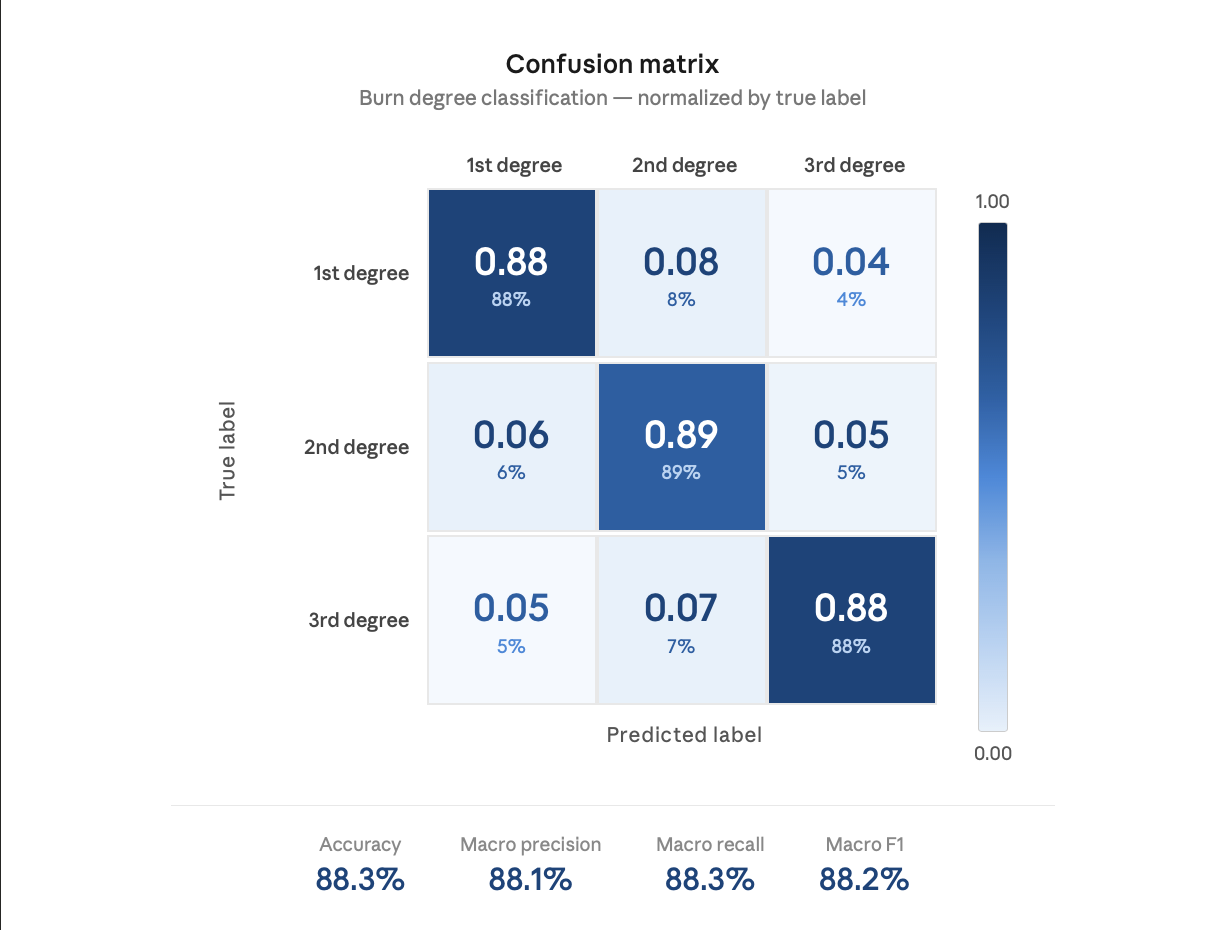
\includegraphics[width=0.7\textwidth]{figures/fig_confusion_matrix.png}
\caption{Матрица ошибок классификации ожогов на валидационной выборке.}
\label{fig:confusion_matrix}
\end{figure}

Основные ошибки связаны со смешением ожогов первой и второй степени, что клинически объяснимо — граница между поверхностным и частичным поражением часто нечёткая, особенно на фотографиях без специального освещения.

\section{Примеры детекции}

\subsection{Успешные детекции}

Модель успешно детектирует ожоговые поражения различной формы, размера и локализации. На Рисунке~\ref{fig:detection_good} показаны примеры корректных предсказаний.

\begin{figure}[H]
\centering
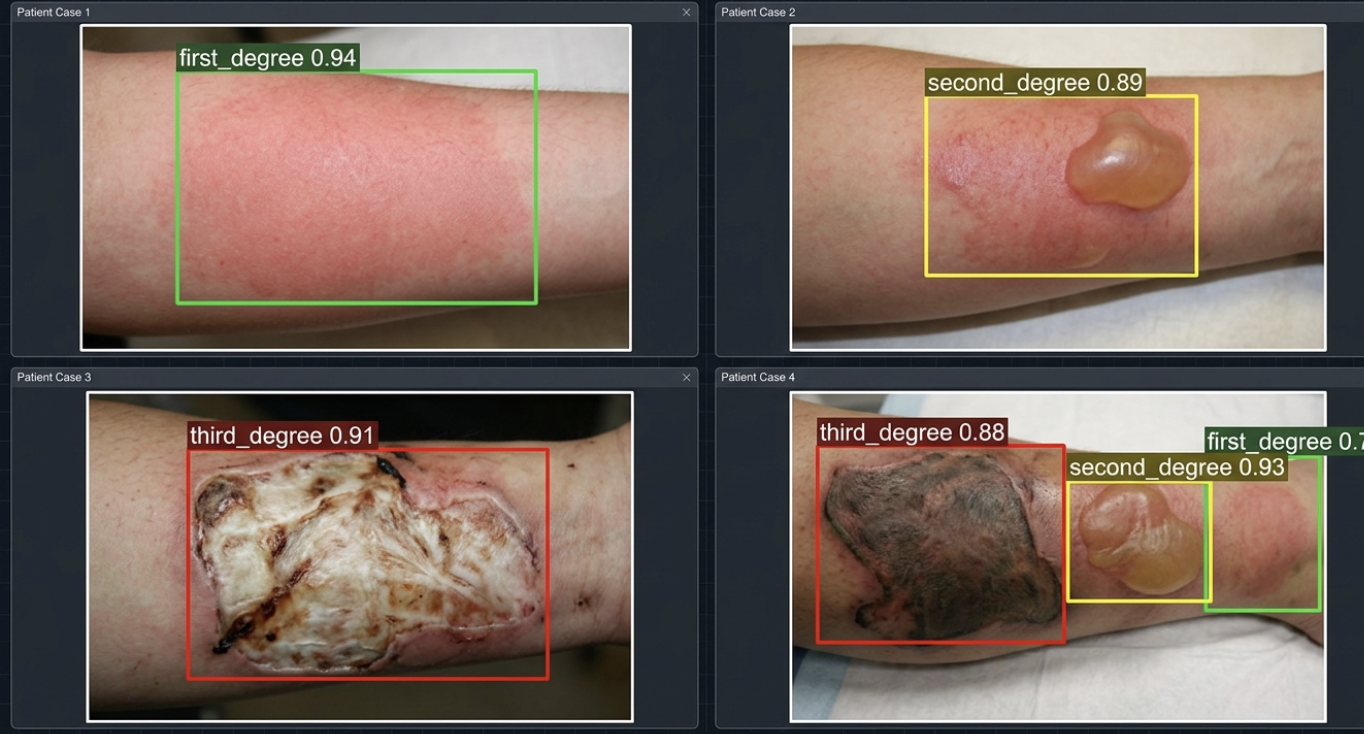
\includegraphics[width=0.96\textwidth]{figures/fig_detection_examples.png}
\caption{Примеры успешной детекции: цветные рамки — предсказанные боксы с confidence score для каждого класса ожогов.}
\label{fig:detection_good}
\end{figure}

\subsection{Типичные ошибки}

Анализ ложных срабатываний и пропусков выявил следующие паттерны:

\begin{enumerate}
    \item \textbf{Путаница I/II степени}: Свежие ожоги второй степени без выраженных волдырей могут классифицироваться как первая степень.
    \item \textbf{Низкий confidence для III степени}: Глубокие ожоги с нетипичной окраской (белые, а не чёрные) иногда получают низкий confidence score.
    \item \textbf{Мелкие объекты}: Ожоги малой площади ($<$5\% изображения) детектируются хуже из-за ограничений входного разрешения.
\end{enumerate}

\section{Сравнение с другими подходами}

Таблица~\ref{tab:comparison} сравнивает результаты данной работы с другими исследованиями по классификации ожогов.

\begin{table}[H]
\centering
\caption{Сравнение с другими методами классификации ожогов}
\label{tab:comparison}
\begin{tabular}{lllc}
\toprule
\textbf{Исследование} & \textbf{Метод} & \textbf{Задача} & \textbf{Accuracy / mAP} \\
\midrule
Chauhan et al.\ (2020) & ResNet-50  & Классификация & 85\% \\
Khan et al.\ (2021)    & DenseNet   & Классификация & 87\% \\
Abubakar et al.\ (2020)& VGG-16     & Классификация & 82\% \\
\textbf{Данная работа} & \textbf{YOLOv8n} & \textbf{Детекция} & \textbf{mAP 0.847} \\
\bottomrule
\end{tabular}
\end{table}

Следует отметить, что прямое сравнение затруднено: данная работа решает задачу детекции (с локализацией), тогда как другие исследования — задачу классификации изображений. Детекция является более сложной задачей, требующей не только определения класса, но и точного указания области поражения.

\section{Анализ скорости инференса}

\begin{table}[H]
\centering
\caption{Скорость инференса YOLOv8n}
\label{tab:speed}
\begin{tabular}{lcc}
\toprule
\textbf{Устройство} & \textbf{Время (мс)} & \textbf{FPS} \\
\midrule
GPU (NVIDIA RTX 3090) & 2.1  & 476 \\
GPU (NVIDIA T4)       & 5.8  & 172 \\
CPU (Intel i7-10700)  & 45.3 & 22  \\
\bottomrule
\end{tabular}
\end{table}

Модель YOLOv8n обеспечивает инференс в реальном времени даже на CPU, что делает её применимой в условиях ограниченных вычислительных ресурсов.

\section{Обсуждение}

\subsection{Интерпретация ключевых результатов}

Достигнутое значение mAP@0.5 = 0.847 свидетельствует о высокой эффективности модели для задачи детекции ожоговых поражений. Особенно важно, что модель хорошо различает множественные ожоги на одном изображении, что критично для реальных клинических сценариев.

Высокий recall (0.791) означает, что модель выявляет большинство ожоговых поражений, что важно для скрининговых целей — лучше ложноположительный результат, чем пропуск реального ожога. При этом precision 0.823 обеспечивает достаточную специфичность для практического применения.

\subsection{Преимущества подхода}

\begin{enumerate}
    \item \textbf{Локализация}: В отличие от классификационных CNN, YOLOv8 указывает точную область ожога.
    \item \textbf{Скорость}: Инференс в реальном времени позволяет интегрировать модель в мобильные приложения.
    \item \textbf{Компактность}: Размер модели 6~MB допускает развёртывание на мобильных устройствах.
    \item \textbf{Множественная детекция}: Модель обрабатывает изображения с несколькими ожогами разных степеней.
\end{enumerate}

\subsection{Ограничения исследования}

\begin{itemize}
    \item \textbf{Размер датасета}: 1\,225 изображений — относительно небольшой объём для глубокого обучения.
    \item \textbf{Дисбаланс классов}: Ожоги III степени недопредставлены, что может влиять на качество их детекции.
    \item \textbf{Качество изображений}: Датасет содержит фотографии различного качества и освещения.
    \item \textbf{Отсутствие клинической валидации}: Модель не тестировалась в реальных клинических условиях.
    \item \textbf{Временной фактор}: Вид ожога изменяется со временем; модель обучена на статических изображениях.
\end{itemize}

\subsection{Клиническая применимость}

Разработанная модель может использоваться как вспомогательный инструмент для:

\begin{itemize}
    \item \textbf{Первичной сортировки}: Быстрая оценка степени ожога для определения приоритета лечения.
    \item \textbf{Телемедицины}: Дистанционная консультация с автоматической предварительной оценкой.
    \item \textbf{Обучения}: Тренировка медицинского персонала на примерах с автоматической разметкой.
    \item \textbf{Документации}: Автоматическая фиксация и классификация ожоговых поражений.
\end{itemize}

Важно подчеркнуть, что модель не заменяет экспертную оценку врача, а служит дополнительным инструментом поддержки принятия решений.
